\documentclass[tikz,border=3pt]{standalone}
\usepackage{amsmath}
\usepackage{tikz}
\usetikzlibrary{calc}
\begin{document}
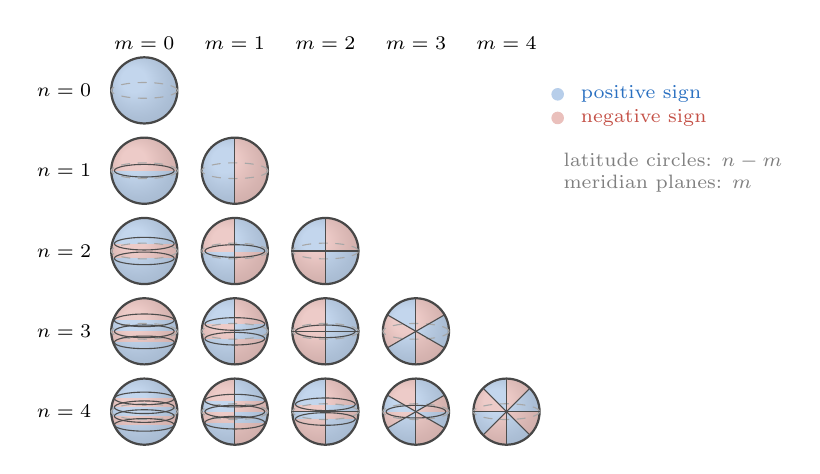
\begin{tikzpicture}[font=\scriptsize, line cap=round, line join=round]
  \definecolor{pos}{RGB}{42,112,193}
  \definecolor{neg}{RGB}{196,80,70}
  \definecolor{grid}{RGB}{95,95,95}

  \newcommand{\harmonicglyph}[4]{%
    \begin{scope}[shift={(#1,#2)}]
      \pgfmathtruncatemacro{\N}{#3}
      \pgfmathtruncatemacro{\M}{#4}
      \pgfmathtruncatemacro{\Lat}{#3-#4}
      \pgfmathtruncatemacro{\Bands}{\Lat+1}
      \begin{scope}
        \clip (0,0) circle (0.42);
        \ifnum\M=0
          \foreach \j in {0,...,\Lat} {
            \pgfmathsetmacro{\ya}{-0.28 + 0.56*\j/\Bands}
            \pgfmathsetmacro{\yb}{-0.28 + 0.56*(\j+1)/\Bands}
            \ifnum\j=0
              \pgfmathsetmacro{\ya}{-0.48}
            \fi
            \ifnum\j=\Lat
              \pgfmathsetmacro{\yb}{0.48}
            \fi
            \ifodd\j
              \fill[neg!36] (-0.48,\ya) rectangle (0.48,\yb);
            \else
              \fill[pos!34] (-0.48,\ya) rectangle (0.48,\yb);
            \fi
          }
        \else
          \pgfmathtruncatemacro{\Sectors}{2*\M}
          \pgfmathtruncatemacro{\LastSector}{\Sectors-1}
          \foreach \j in {0,...,\Lat} {
            \pgfmathsetmacro{\ya}{-0.28 + 0.56*\j/\Bands}
            \pgfmathsetmacro{\yb}{-0.28 + 0.56*(\j+1)/\Bands}
            \ifnum\j=0
              \pgfmathsetmacro{\ya}{-0.48}
            \fi
            \ifnum\j=\Lat
              \pgfmathsetmacro{\yb}{0.48}
            \fi
            \begin{scope}
              \clip (-0.48,\ya) rectangle (0.48,\yb);
              \foreach \i in {0,...,\LastSector} {
                \pgfmathsetmacro{\a}{90 + \i*360/\Sectors}
                \pgfmathsetmacro{\b}{90 + (\i+1)*360/\Sectors}
                \pgfmathtruncatemacro{\Parity}{mod(\i+\j,2)}
                \ifodd\Parity
                  \fill[neg!36] (0,0) -- (\a:0.58)
                    arc[start angle=\a,end angle=\b,radius=0.58] -- cycle;
                \else
                  \fill[pos!34] (0,0) -- (\a:0.58)
                    arc[start angle=\a,end angle=\b,radius=0.58] -- cycle;
                \fi
              }
            \end{scope}
          }
        \fi
      \end{scope}
      \shade[ball color=white,opacity=0.18] (0,0) circle (0.42);
      \draw[black!72,thick] (0,0) circle (0.42);
      \draw[grid!55,thin,dashed] (0,0) ellipse (0.42 and 0.10);
      \ifnum\Lat>0
        \foreach \j in {1,...,\Lat} {
          \pgfmathsetmacro{\yy}{-0.28 + 0.56*\j/\Bands}
          \draw[black!70,thin] (0,\yy) ellipse (0.38 and 0.08);
        }
      \fi
      \ifnum\M>0
        \pgfmathtruncatemacro{\LastMeridian}{\M-1}
        \foreach \j in {0,...,\LastMeridian} {
          \pgfmathsetmacro{\ang}{90 + \j*180/\M}
          \draw[black!70,thin] ({0.42*cos(\ang)},{0.42*sin(\ang)}) --
                               ({-0.42*cos(\ang)},{-0.42*sin(\ang)});
        }
      \fi
    \end{scope}%
  }

  \foreach \m in {0,...,4} {
    \node[font=\scriptsize] at ({1.15*\m},0.60) {$m=\m$};
  }
  \foreach \n in {0,...,4} {
    \node[font=\scriptsize,anchor=east] at (-0.55,{-1.02*\n}) {$n=\n$};
  }

  \harmonicglyph{0}{0}{0}{0}
  \harmonicglyph{0}{-1.02}{1}{0}
  \harmonicglyph{1.15}{-1.02}{1}{1}
  \harmonicglyph{0}{-2.04}{2}{0}
  \harmonicglyph{1.15}{-2.04}{2}{1}
  \harmonicglyph{2.30}{-2.04}{2}{2}
  \harmonicglyph{0}{-3.06}{3}{0}
  \harmonicglyph{1.15}{-3.06}{3}{1}
  \harmonicglyph{2.30}{-3.06}{3}{2}
  \harmonicglyph{3.45}{-3.06}{3}{3}
  \harmonicglyph{0}{-4.08}{4}{0}
  \harmonicglyph{1.15}{-4.08}{4}{1}
  \harmonicglyph{2.30}{-4.08}{4}{2}
  \harmonicglyph{3.45}{-4.08}{4}{3}
  \harmonicglyph{4.60}{-4.08}{4}{4}

  \fill[pos!34] (5.25,-0.05) circle (0.08);
  \node[anchor=west,text=pos] at (5.42,-0.05) {positive sign};
  \fill[neg!36] (5.25,-0.35) circle (0.08);
  \node[anchor=west,text=neg] at (5.42,-0.35) {negative sign};
  \node[anchor=west,align=left,text=grid!80] at (5.20,-1.05)
    {latitude circles: $n-m$\\meridian planes: $m$};
\end{tikzpicture}
\end{document}
